\documentclass[usenames,dvipsnames]{beamer}
\usepackage{../../shared/styles/custom}
\usepackage{../../shared/styles/conventions}

\title{Decision Trees}
\date{\today}
\author{Nipun Batra and teaching staff}
\institute{IIT Gandhinagar}

% Pop quiz counter is defined globally in theme-nipun.sty
\setcounter{popquiz}{0}

\begin{document}
\maketitle

% Table of Contents
\begin{frame}{Table of Contents}
    \small
    \tableofcontents[hideallsubsections]
\end{frame}

\section{Introduction and Motivation}
	
\begin{frame}{The need for interpretability}
\begin{figure}
    \centering
    \includegraphics[scale=0.29]{../assets/decision-trees/diagrams/interpretability}
    \label{fig:interpretability}
\end{figure}
	
\end{frame}
	
\renewcommand{\arraystretch}{0.85}

\begin{frame}{Training Data}
\begin{center}    
\begin{tabular}{lllll||l} \toprule
\textbf{Day} & \textbf{Outlook}  & \textbf{Temp} & \textbf{Humidity} & \textbf{Windy}  & \textbf{Play} \\ \midrule
D1  & Sunny    & Hot  & High     & Weak   & No   \\
D2  & Sunny    & Hot  & High     & Strong & No   \\
D3  & Overcast & Hot  & High     & Weak   & Yes  \\
D4  & Rain     & Mild & High     & Weak   & Yes  \\
D5  & Rain     & Cool & Normal   & Weak   & Yes  \\
D6  & Rain     & Cool & Normal   & Strong & No   \\
D7  & Overcast & Cool & Normal   & Strong & Yes  \\
D8  & Sunny    & Mild & High     & Weak   & No   \\
D9  & Sunny    & Cool & Normal   & Weak   & Yes  \\
D10 & Rain     & Mild & Normal   & Weak   & Yes  \\
D11 & Sunny    & Mild & Normal   & Strong & Yes  \\
D12 & Overcast & Mild & High     & Strong & Yes  \\
D13 & Overcast & Hot  & Normal   & Weak   & Yes  \\
D14 & Rain     & Mild & High     & Strong & No  \\ \bottomrule
\end{tabular}
\end{center}
\end{frame}

\begin{frame}{Learning a Complicated Neural Network}
\begin{center}
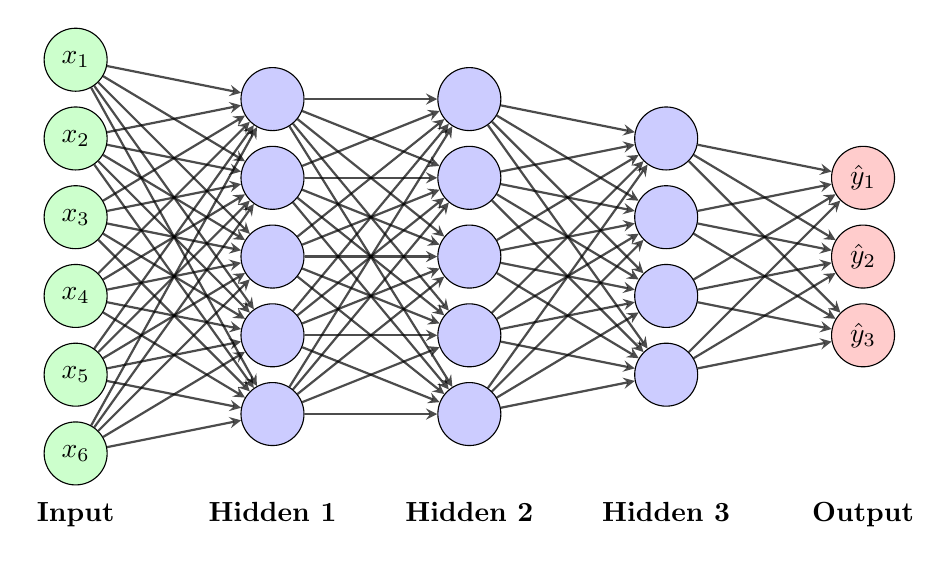
\begin{tikzpicture}[
	node distance=1.5cm and 2cm,
	neuron/.style={circle, draw, minimum size=0.8cm, inner sep=0pt, fill=blue!20},
	input/.style={circle, draw, minimum size=0.8cm, inner sep=0pt, fill=green!20},
	output/.style={circle, draw, minimum size=0.8cm, inner sep=0pt, fill=red!20},
	connection/.style={->, >=stealth, thick, opacity=0.7}
	]
	
	% Input layer (6 nodes)
	\foreach \y in {1,2,3,4,5,6}
		\node[input] (i\y) at (0, 6-\y) {$x_\y$};
	
	% Hidden layer 1 (5 nodes)
	\foreach \y in {1,2,3,4,5}
		\node[neuron] (h1\y) at (2.5, 5.5-\y) {};
	
	% Hidden layer 2 (5 nodes) 
	\foreach \y in {1,2,3,4,5}
		\node[neuron] (h2\y) at (5, 5.5-\y) {};
	
	% Hidden layer 3 (4 nodes)
	\foreach \y in {1,2,3,4}
		\node[neuron] (h3\y) at (7.5, 5-\y) {};
	
	% Output layer (3 nodes)
	\foreach \y in {1,2,3}
		\node[output] (o\y) at (10, 4.5-\y) {$\hat{y}_\y$};
	
	% Connections: Input to Hidden1
	\foreach \i in {1,2,3,4,5,6} {
		\foreach \j in {1,2,3,4,5} {
			\draw[connection] (i\i) -- (h1\j);
		}
	}
	
	% Connections: Hidden1 to Hidden2
	\foreach \i in {1,2,3,4,5} {
		\foreach \j in {1,2,3,4,5} {
			\draw[connection] (h1\i) -- (h2\j);
		}
	}
	
	% Connections: Hidden2 to Hidden3
	\foreach \i in {1,2,3,4,5} {
		\foreach \j in {1,2,3,4} {
			\draw[connection] (h2\i) -- (h3\j);
		}
	}
	
	% Connections: Hidden3 to Output
	\foreach \i in {1,2,3,4} {
		\foreach \j in {1,2,3} {
			\draw[connection] (h3\i) -- (o\j);
		}
	}
	
	% Layer labels
	\node[below] at (0, -0.5) {\textbf{Input}};
	\node[below] at (2.5, -0.5) {\textbf{Hidden 1}};
	\node[below] at (5, -0.5) {\textbf{Hidden 2}};
	\node[below] at (7.5, -0.5) {\textbf{Hidden 3}};
	\node[below] at (10, -0.5) {\textbf{Output}};
	
\end{tikzpicture}
\end{center}

%\textbf{Complex model, same evaluation:} Even with this intricate network, we still use the same accuracy metrics to evaluate performance!
\end{frame}

\begin{frame}{Learnt Decision Tree}
\begin{tikzpicture}[
node/.style={%
	draw,
	rectangle,
},
]

\node [node] (A) {Outlook};
\path (A) ++(-150:\nodeDist) node [node] (B) {Humidity};
\path (A) ++(-90:\nodeDist/2) node [node, fill=green] (C) {Yes};
\path (A) ++(-30:\nodeDist) node [node] (D) {Wind};
\path (B) ++(-135:\nodeDist) node [node, fill=red] (E) {No};
\path (B) ++(-45:\nodeDist) node [node, fill=green] (F) {Yes};
\path (D) ++(-45:\nodeDist) node [node, fill=red] (G) {No};
\path (D) ++(-135:\nodeDist) node [node, fill=green] (H) {Yes};

\draw (A) -- (B) node [left,pos=0.25] {Sunny}(A);
\draw (A) -- (C) node [right,pos=0.8] {Overcast}(A);
\draw (A) -- (D) node [right,pos=0.5] {Rain}(A);
\draw (B) -- (E) node [left,pos=0.25] {High}(A);
\draw (B) -- (F) node [right,pos=0.25] {Normal}(C);
\draw (D) -- (G) node [right,pos=0.25] {Strong}(A);
\draw (D) -- (H) node [left,pos=0.25] {Weak}(A);
\end{tikzpicture}

\end{frame}

\begin{frame}{Medical Diagnosis using Decision Trees }
\begin{figure}
	\centering
	\includegraphics[width=1\linewidth]{../assets/decision-trees/diagrams/decision-medical}
	\caption{Source: Improving medical decision trees by combining relevant health-care criteria}
	\label{fig:decision-medical}
\end{figure}

\end{frame}

\begin{frame}{Leo Breiman (1928-2005)}
\begin{center}
\begin{figure}
	\centering
	\includegraphics[width=1.1\linewidth]{../assets/decision-trees/diagrams/brieman}
	\label{fig:brieman}
\end{figure}
\end{center}
\end{frame}

\begin{frame}{Leo Breiman: Revolutionary Contributions to ML}
\begin{keypointsbox}{Major Algorithmic Breakthroughs:}
\cleanitemize{
    \item \textbf{CART (1984)}: Classification and Regression Trees
    \item \textbf{Bagging (1994)}: Bootstrap Aggregating
    \item \textbf{Random Forests (2001)}: Ensemble of Decision Trees
    \item \textbf{Two Cultures (2001)}: Data Modeling vs. Algorithmic Modeling
}
\end{keypointsbox}
\end{frame}


\begin{frame}{Computational Complexity Classes: A Quick Primer}
\scriptsize
\begin{definitionbox}{Key Complexity Classes}
\cleanitemize{
    \item \textbf{P}: Problems solvable in polynomial time
    \cleanitemize{
        \item Example: Sorting $n$ numbers in $O(n \log n)$ time
    }
    \item \textbf{NP}: Problems where solutions can be \emph{verified} in polynomial time
    \cleanitemize{
        \item Example: Given a sudoku solution, verify it's correct
    }
    \item \textbf{NP-Complete}: Hardest problems in NP 
    \cleanitemize{
        \item Both in NP and at least as hard as any NP problem
        \item Example: Boolean satisfiability (SAT)
    }
    \item \textbf{NP-Hard}: At least as hard as NP-Complete problems
    \cleanitemize{
        \item May not be in NP (solutions might not be verifiable quickly)
        \item Example: Optimization versions of NP-Complete problems
    }
}
\end{definitionbox}
\end{frame}

\begin{frame}{Finding the Optimal Decision Tree}
\begin{center}
\begin{figure}
\centering
\includegraphics[width=0.8\linewidth]{../assets/decision-trees/diagrams/NP-hard}
\label{fig:np-hard}
\end{figure}
\end{center}
\textbf{The Problem}: Given training data, find the decision tree with the highest accuracy
\end{frame}

\begin{frame}{Optimal Decision Trees are NP-Complete}
\begin{alertbox}{Computational Complexity}
\textbf{Finding optimal decision tree is NP-Complete}
\cleanitemize{
    \item \textbf{Verification}: Given a tree, check its accuracy quickly \checkmark
    \item \textbf{Construction}: Exponentially many trees to check \crossmark
}
\end{alertbox}

\onslide<3->{
\begin{examplebox}{What This Means}
    \cleanitemize{
        \item No efficient algorithm exists (unless P = NP)
        \item Must use heuristics like greedy algorithms
        \item ID3, C4.5, CART use greedy approaches
        \item Good solutions, but no optimality guarantee
    }
\end{examplebox}
}
\end{frame}


\begin{frame}{Greedy Algorithm}
Core idea: At each level, choose an attribute that gives
\textbf{biggest estimated} performance gain!

\begin{figure}
	\centering
	\includegraphics[width=0.8\linewidth]{../assets/decision-trees/diagrams/gredy}
	\caption{Greedy $\neq$ Optimal}
	\label{fig:gredy}
\end{figure}
\end{frame}


\section{Discrete Input, Discrete Output}

\begin{frame}{Towards biggest estimated performance gain}
\begin{columns}
\begin{column}{.7\textwidth}
\begin{scriptsize}
\begin{tabular}{lllll||l} \toprule
\textbf{Day} & \textbf{Outlook}  & \textbf{Temp} & \textbf{Humidity} & \textbf{Windy}  & \textbf{Play} \\ \midrule
D1  & Sunny    & Hot  & High     & Weak   & No   \\
D2  & Sunny    & Hot  & High     & Strong & No   \\
D3  & Overcast & Hot  & High     & Weak   & Yes  \\
D4  & Rain     & Mild & High     & Weak   & Yes  \\
D5  & Rain     & Cool & Normal   & Weak   & Yes  \\
D6  & Rain     & Cool & Normal   & Strong & No   \\
D7  & Overcast & Cool & Normal   & Strong & Yes  \\
D8  & Sunny    & Mild & High     & Weak   & No   \\
D9  & Sunny    & Cool & Normal   & Weak   & Yes  \\
D10 & Rain     & Mild & Normal   & Weak   & Yes  \\
D11 & Sunny    & Mild & Normal   & Strong & Yes  \\
D12 & Overcast & Mild & High     & Strong & Yes  \\
D13 & Overcast & Hot  & Normal   & Weak   & Yes  \\
D14 & Rain     & Mild & High     & Strong & No  \\ \bottomrule
\end{tabular}
\end{scriptsize}
\end{column}
\onslide<2->{\begin{column}{0.4\textwidth}
\begin{scriptsize}
\cleanitemize{
    \item For examples, we have 9 Yes, 5 No   
    \item Would it be trivial if we had 14 Yes or 14 No?
    \item Yes!
    \item Key insight: Problem is ``easier'' when there is less disagreement
    \item Need some statistical measure of ``disagreement'' 
}
\end{scriptsize}
\end{column}}
\end{columns}
\end{frame}


\begin{frame}{Claude Shannon (1948): The Birth of Information Theory}
\begin{definitionbox}{The Big Idea}
Information is inversely related to probability. \textbf{Rare events are more informative!}
\end{definitionbox}
\pause
\textbf{Think about it:} Which headline tells you more?
\pause
\cleanitemize{
\item ``The sun rose this morning''
\item ``It snowed in Gandhinagar in July''
}

\onslide<5->{
The second one! Because it's \textbf{unexpected}.\\
\textbf{Shannon's insight:} The amount of information in an event should be inversely proportional to its probability.}
\end{frame}

\begin{frame}{Measuring Surprise: Step by Step}
\textbf{Shannon's Information Formula:}
$$I(x) = -\log_2 p(x)$$

\pause
\textbf{Why the negative log?}
\cleanitemize{
\item Probabilities are between 0 and 1
\item $\log_2$ of values $< 1$ gives negative numbers
\item We want information to be positive
\item Hence the negative sign!
}

\onslide<6->{
\textbf{Why base 2?} So information is measured in \textbf{bits}.}
\end{frame}

\begin{frame}{Calculating Surprise: Detailed Examples}
\textbf{Example 1: Summer weather in Phoenix}
\cleanitemize{
\item Sunny day: $p = 0.9$
\item Information: $I = -\log_2(0.9) = -(-0.152) = 0.152$ bits
\item \textcolor{blue}{\textbf{Low surprise}} - we expect sunny weather
}

\onslide<4->{
\textbf{Example 2: Snow in Phoenix in July}}
\cleanitemize{
\item Probability: $p = 0.0001$ (extremely rare!)
\item Information: $I = -\log_2(0.0001) = -(-13.29) = 13.29$ bits
\item \textcolor{red}{\textbf{High surprise}} - this would be shocking news!
}

\onslide<7->{
\textbf{Notice:} Rare events carry $\sim$90× more information!}
\end{frame}

\begin{frame}{From Single Events to Distributions}
\textbf{Question:} What if we have multiple possible outcomes?

\pause
\textbf{Example:} Weather in Delhi (4 possibilities)
\cleanitemize{
\item Rainy: $p = 0.5$
\item Cloudy: $p = 0.3$  
\item Sunny: $p = 0.15$
\item Snowy: $p = 0.05$
}

\onslide<6->{
\textbf{Problem:} Each day gives different amounts of information!}
\cleanitemize{
\item If it's rainy: $I = -\log_2(0.5) = 1.0$ bit
\item If it's sunny: $I = -\log_2(0.15) = 2.74$ bits  
\item If it's snowy: $I = -\log_2(0.05) = 4.32$ bits
}

\onslide<9->{
\textbf{Solution:} Take the \textbf{expected} (average) information!}
\end{frame}

\begin{frame}{Entropy: Expected Information}
\begin{definitionbox}{Entropy Formula}
$$H(X) = \mathbb{E}[I(X)] = -\sum_{i} p(x_i) \log_2 p(x_i)$$
\textbf{Entropy} = Expected amount of information per observation
\end{definitionbox}

\pause
\textbf{Delhi weather calculation:}
\pause
\begin{align*}
\uncover<+-> {H &= -p(\text{rain}) \log_2 p(\text{rain}) - p(\text{cloudy}) \log_2 p(\text{cloudy})\\
&\quad - p(\text{sunny}) \log_2 p(\text{sunny}) - p(\text{snow}) \log_2 p(\text{snow})}\\
\uncover<+-> { &= -0.5 \log_2(0.5) - 0.3 \log_2(0.3) - 0.15 \log_2(0.15) - 0.05 \log_2(0.05)}\\
\uncover<+-> { &= 0.5(1.0) + 0.3(1.74) + 0.15(2.74) + 0.05(4.32)}\\
\uncover<+-> { &= 0.5 + 0.52 + 0.41 + 0.22 = \mathbf{1.65} \text{ bits}}
\end{align*}
\end{frame}

\begin{frame}{Entropy Intuition: Extreme Cases}
\textbf{Case 1: Completely predictable}
\cleanitemize{
\item Desert: Always sunny ($p = 1.0$)
\item $H = -1.0 \log_2(1.0) = -1.0 \times 0 = \mathbf{0}$ bits
\item \textcolor{blue}{\textbf{Zero entropy}} = No surprise = Completely predictable
}
\onslide<4->{\textbf{Case 2: Maximum uncertainty}}
\cleanitemize{
\item Fair coin: Heads/Tails equally likely ($p = 0.5$ each)
\item $H = -0.5 \log_2(0.5) - 0.5 \log_2(0.5) = 0.5(1) + 0.5(1) = \mathbf{1.0}$ bit
\item \textcolor{red}{\textbf{Maximum entropy}} = Maximum surprise = Completely unpredictable
}
\onslide<7->{\textbf{Key insight:} Entropy ranges from 0 (certain) to $\log_2(n)$ (uniform over $n$ outcomes)}
\end{frame}

\begin{frame}{Entropy in Decision Trees: The Connection}
\textbf{Why do we care about entropy in ML?}
\pause
\begin{examplebox}{Decision Tree Goal}
We want to split data into \textbf{pure} subsets where we can make confident predictions.
\end{examplebox}

\pause
\cleanitemize{
\item \textbf{Pure node}: All examples same class → \textcolor{blue}{Low entropy} → \textcolor{blue}{Good split}
\item \textbf{Mixed node}: Examples from different classes → \textcolor{red}{High entropy} → \textcolor{red}{Bad split}
}

\onslide<5->{\textbf{Strategy:} Choose splits that \textbf{reduce entropy} the most! This is exactly what \textbf{Information Gain} measures.}
\end{frame}

\begin{frame}{Entropy}
 Statistical measure to characterize the
(im)purity of examples

\pause $H(X) = -\sum_{i=1}^k p(x_i) \log_2 p(x_i)$

\begin{figure}[htp]
    \centering
    \begin{notebookbox}{https://nipunbatra.github.io/ml-teaching/notebooks/entropy.html}
      \includegraphics[scale=0.6]{../assets/decision-trees/figures/entropy.pdf}
    \end{notebookbox}
  \end{figure}

\end{frame}
	
\begin{frame}{Towards biggest estimated performance gain}
\begin{columns}[T,onlytextwidth]
    \begin{column}{.7\textwidth}
        \begin{scriptsize}
            \begin{tabular}{lllll||l} \toprule
                \textbf{Day} & \textbf{Outlook}  & \textbf{Temp} & \textbf{Humidity} & \textbf{Windy}  & \textbf{Play} \\ \midrule
                D1  & Sunny    & Hot  & High     & Weak   & No   \\
                D2  & Sunny    & Hot  & High     & Strong & No   \\
                D3  & Overcast & Hot  & High     & Weak   & Yes  \\
                D4  & Rain     & Mild & High     & Weak   & Yes  \\
                D5  & Rain     & Cool & Normal   & Weak   & Yes  \\
                D6  & Rain     & Cool & Normal   & Strong & No   \\
                D7  & Overcast & Cool & Normal   & Strong & Yes  \\
                D8  & Sunny    & Mild & High     & Weak   & No   \\
                D9  & Sunny    & Cool & Normal   & Weak   & Yes  \\
                D10 & Rain     & Mild & Normal   & Weak   & Yes  \\
                D11 & Sunny    & Mild & Normal   & Strong & Yes  \\
                D12 & Overcast & Mild & High     & Strong & Yes  \\
                D13 & Overcast & Hot  & Normal   & Weak   & Yes  \\
                D14 & Rain     & Mild & High     & Strong & No  \\ \bottomrule
            \end{tabular}
        \end{scriptsize}
    \end{column}

    \begin{column}{0.4\textwidth}
        \begin{scriptsize}
            \cleanitemize{
                \item Can we use Outlook as the root node?
                \item When Outlook is overcast, we always Play and thus no ``disagreement''
            }
        \end{scriptsize}
    \end{column}
\end{columns}
\end{frame}
	
\begin{frame}{Information Gain}
 Reduction in entropy
by partitioning examples (S) on attribute A
$$
\operatorname{Gain}(S, A) \equiv \text{Entropy}(S)-\sum_{v \in \text{Values}(A)} \frac{|S_{v}|}{|S|} \text{Entropy}(S_{v})
$$
\end{frame}

\popquiz{
\textbf{What does entropy measure in the context of decision trees?}

\begin{enumerate}[A)]
  \item The depth of the tree
  \item The impurity or ``disagreement'' in a set of examples
  \item The number of features in the dataset
  \item The accuracy of the tree
\end{enumerate}
}{
{\color{magenta}\textbf{B) The impurity or ``disagreement'' in a set of examples}} — Higher entropy means more mixed classes, lower entropy means more pure subsets.
}


\begin{frame}{ID3 (Examples, Target Attribute, Attributes)}
\cleanitemize{
	\item Create a root node for tree
	\item If all examples are +/-, return root with label = +/-
	\item  If attributes = empty, return root with most common value of
	Target Attribute in Examples
	\item Begin
	\cleanitemize{
		\item A $\leftarrow$ attribute from Attributes which best classifies
		Examples
		\item 	Root $\leftarrow$ A
		\item  For each value (v) of A
		\cleanitemize{
			\item Add new tree branch : A = v
			\item  Examples\textsubscript{v}: subset of examples that A = v
			\item If Examples\textsubscript{v}is empty: add leaf with label = most
			common value of Target Attribute
			\item Else: ID3 (Examples\textsubscript{v}, Target attribute, Attributes - {A})
		}
	}


}
\end{frame}

	\begin{frame}{Training Data}
\begin{tabular}{lllll||l} \toprule
	\textbf{Day} & \textbf{Outlook}  & \textbf{Temp} & \textbf{Humidity} & \textbf{Windy}  & \textbf{Play} \\ \midrule
	D1  & Sunny    & Hot  & High     & Weak   & No   \\
	D2  & Sunny    & Hot  & High     & Strong & No   \\
	D3  & Overcast & Hot  & High     & Weak   & Yes  \\
	D4  & Rain     & Mild & High     & Weak   & Yes  \\
	D5  & Rain     & Cool & Normal   & Weak   & Yes  \\
	D6  & Rain     & Cool & Normal   & Strong & No   \\
	D7  & Overcast & Cool & Normal   & Strong & Yes  \\
	D8  & Sunny    & Mild & High     & Weak   & No   \\
	D9  & Sunny    & Cool & Normal   & Weak   & Yes  \\
	D10 & Rain     & Mild & Normal   & Weak   & Yes  \\
	D11 & Sunny    & Mild & Normal   & Strong & Yes  \\
	D12 & Overcast & Mild & High     & Strong & Yes  \\
	D13 & Overcast & Hot  & Normal   & Weak   & Yes  \\
	D14 & Rain     & Mild & High     & Strong & No  \\ \bottomrule
\end{tabular}
\end{frame}


\begin{frame}{Entropy calculated}
We have 14 examples in $S$: 5 No, 9 Yes

$$\Entropy(S) = -p_{\text{No}} \log_2 p_{\text{No}} - p_{\text{Yes}} \log_2 p_{\text{Yes}}$$
$$
= -\frac{5}{14} \log_2\left(\frac{5}{14}\right) - \frac{9}{14} \log_2\left(\frac{9}{14}\right) = 0.940
$$
\end{frame}

\begin{frame}{Information Gain for Outlook}
\begin{tabular}{l|l} \toprule
\textbf{Outlook} & \textbf{Play} \\ \midrule
Sunny    & No   \\
Sunny    & No   \\
Overcast & Yes  \\
Rain     & Yes  \\
Rain     & Yes  \\
Rain     & No   \\
Overcast & Yes  \\
Sunny    & No   \\
Sunny    & Yes  \\
Rain     & Yes  \\
Sunny    & Yes  \\
Overcast & Yes  \\
Overcast & Yes  \\
Rain     & No  \\ \bottomrule
\end{tabular}
\end{frame}

\begin{frame}{Information Gain for Outlook}
\begin{columns}

\begin{column}{.32\textwidth}
	\begin{table}
\begin{tabular}{l|l} \toprule
	\textbf{Outlook} & \textbf{Play} \\ \midrule
	Sunny    & No   \\
	Sunny    & No   \\
	Sunny    & No   \\
	Sunny    & Yes  \\
	Sunny    & Yes  \\

\bottomrule
\end{tabular}
We have 2 Yes, 3 No
$\Entropy = -\frac{3}{5} \log_2\left(\frac{3}{5}\right) - \frac{2}{5} \log_2\left(\frac{2}{5}\right) = 0.971$
\end{table}
\end{column}

\onslide<2->{
\begin{column}{.32\textwidth}
	\begin{table}
\begin{tabular}{l|l} \toprule
	\textbf{Outlook} & \textbf{Play} \\ \midrule

	Overcast & Yes  \\
	Overcast & Yes  \\
	Overcast & Yes  \\
	Overcast & Yes  \\ \bottomrule

\end{tabular}
We have 4 Yes, 0 No
$\Entropy = 0$ (pure subset)
	\end{table}
\end{column}
}

\onslide<3->{
\begin{column}{.32\textwidth}
	\begin{table}
\begin{tabular}{l|l} \toprule
	\textbf{Outlook} & \textbf{Play} \\ \midrule
	Rain     & Yes  \\
	Rain     & Yes  \\
	Rain     & No   \\
	Rain     & Yes  \\
	Rain     & No  \\ \bottomrule
\end{tabular}
We have 3 Yes, 2 No
$\Entropy = -\frac{3}{5} \log_2\left(\frac{3}{5}\right) - \frac{2}{5} \log_2\left(\frac{2}{5}\right) = 0.971$
\end{table}
\end{column}
}
\end{columns}
\end{frame}

\begin{frame}{Information Gain}
\begin{align*}
\uncover<+->{\operatorname{Gain}(S, \text{Outlook}) 
&= \text{Entropy}(S) - \\
&\quad \sum_{v \in \{\text{Rain, Sunny, Overcast}\}} \frac{|S_{v}|}{|S|} \, \text{Entropy}(S_{v}) \\
\uncover<+-> {&= 0.940 - \frac{5}{14} \times 0.971 
     - \frac{4}{14} \times 0 
     - \frac{5}{14} \times 0.971}} \\
\uncover<+-> {&= 0.940 - 0.347 - 0 - 0.347} \\
\uncover<+-> {&= 0.246}
\end{align*}
\end{frame}

\begin{frame}{Information Gain}


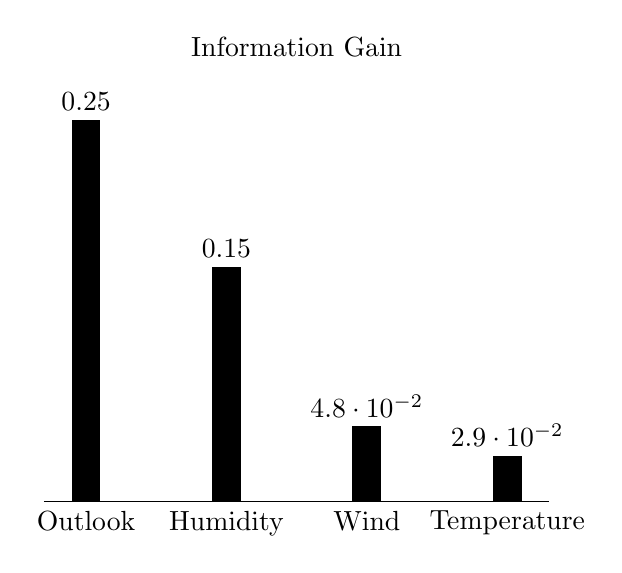
\begin{tikzpicture}
\begin{axis}[
symbolic x coords={Outlook,Humidity,Wind,Temperature},
xtick=data,xtick pos=left, width=8cm,
ytick pos=left,axis x line*=bottom,nodes near coords,hide y axis,title=Information Gain, ymin=0.0]
\addplot[ybar,fill=black] coordinates {
	(Outlook,0.246)
	(Humidity,0.151)
	(Wind,0.048)
	(Temperature,0.029)
};
\end{axis}
\end{tikzpicture}


\end{frame}

\begin{frame}{Learnt Decision Tree}
\begin{tikzpicture}[
node/.style={%
	draw,
	rectangle,
},
]

\node [node] (A) {Outlook};
\path (A) ++(-150:\nodeDist) node [node] (B) {?};
\path (A) ++(-90:\nodeDist/2) node [node, fill=green] (C) {Yes};
\path (A) ++(-30:\nodeDist) node [node] (D) {?};


\draw (A) -- (B) node [left,pos=0.25] {Sunny}(A);
\draw (A) -- (C) node [right,pos=0.8] {Overcast}(A);
\draw (A) -- (D) node [right,pos=0.5] {Rain}(A);

\end{tikzpicture}

\end{frame}

	\begin{frame}{Calling ID3 on Outlook=Sunny}
\begin{tabular}{llll||l} \toprule
	\textbf{Day} & \textbf{Temp} & \textbf{Humidity} & \textbf{Windy}  & \textbf{Play} \\ \midrule
	D1    & Hot  & High     & Weak   & No   \\
	D2     & Hot  & High     & Strong & No   \\
	D8     & Mild & High     & Weak   & No   \\
	D9    & Cool & Normal   & Weak   & Yes  \\
	D11    & Mild & Normal   & Strong & Yes  \\ \bottomrule
\end{tabular}

\cleanitemize{
    \item Gain($S_{\text{Outlook=Sunny}}$, Temp) = Entropy(2 Yes, 3 No) - (2/5)*Entropy(0 Yes, 2 No) -(2/5)*Entropy(1 Yes, 1 No) - (1/5)*Entropy(1 Yes, 0 No) 
    \item Gain($S_{\text{Outlook=Sunny}}$, Humidity) = Entropy(2 Yes, 3 No) - (2/5)*Entropy(2 Yes, 0 No) -(3/5)*Entropy(0 Yes, 3 No) $\implies$ \textbf{maximum possible for the set}
    \item Gain($S_{\text{Outlook=Sunny}}$, Windy) = Entropy(2 Yes, 3 No) - (3/5)*Entropy(1 Yes, 2 No) -(2/5)*Entropy(1 Yes, 1 No) 
}
\end{frame}

\begin{frame}{Learnt Decision Tree}
\begin{tikzpicture}[
node/.style={%
	draw,
	rectangle,
},
]

\node [node] (A) {Outlook};
\path (A) ++(-150:\nodeDist) node [node] (B) {Humidity};
\path (A) ++(-90:\nodeDist/2) node [node, fill=green] (C) {Yes};
\path (A) ++(-30:\nodeDist) node [node] (D) {?};
\path (B) ++(-135:\nodeDist) node [node, fill=red] (E) {No};
\path (B) ++(-45:\nodeDist) node [node, fill=green] (F) {Yes};
;

\draw (A) -- (B) node [left,pos=0.25] {Sunny}(A);
\draw (A) -- (C) node [right,pos=0.8] {Overcast}(A);
\draw (A) -- (D) node [right,pos=0.5] {Rain}(A);
\draw (B) -- (E) node [left,pos=0.25] {High}(A);
\draw (B) -- (F) node [right,pos=0.25] {Normal}(C);

\end{tikzpicture}

\end{frame}


	\begin{frame}{Calling ID3 on (Outlook=Rain)}
\begin{tabular}{llll||l} \toprule
	\textbf{Day}  & \textbf{Temp} & \textbf{Humidity} & \textbf{Windy}  & \textbf{Play} \\ \midrule
	D4    & Mild & High     & Weak   & Yes  \\
	D5     & Cool & Normal   & Weak   & Yes  \\
	D6      & Cool & Normal   & Strong & No   \\
	D10     & Mild & Normal   & Weak   & Yes  \\
	D14      & Mild & High     & Strong & No  \\ \bottomrule
\end{tabular}
\begin{itemize}
	\item The attribute Windy gives the highest information gain
\end{itemize}
\end{frame}

\begin{frame}{Learnt Decision Tree}
\begin{tikzpicture}[
node/.style={%
	draw,
	rectangle,
},
]

\node [node] (A) {Outlook};
\path (A) ++(-150:\nodeDist) node [node] (B) {Humidity};
\path (A) ++(-90:\nodeDist/2) node [node, fill=green] (C) {Yes};
\path (A) ++(-30:\nodeDist) node [node] (D) {Wind};
\path (B) ++(-135:\nodeDist) node [node, fill=red] (E) {No};
\path (B) ++(-45:\nodeDist) node [node, fill=green] (F) {Yes};
\path (D) ++(-45:\nodeDist) node [node, fill=red] (G) {No};
\path (D) ++(-135:\nodeDist) node [node, fill=green] (H) {Yes};

\draw (A) -- (B) node [left,pos=0.25] {Sunny}(A);
\draw (A) -- (C) node [right,pos=0.8] {Overcast}(A);
\draw (A) -- (D) node [right,pos=0.5] {Rain}(A);
\draw (B) -- (E) node [left,pos=0.25] {High}(A);
\draw (B) -- (F) node [right,pos=0.25] {Normal}(C);
\draw (D) -- (G) node [right,pos=0.25] {Strong}(A);
\draw (D) -- (H) node [left,pos=0.25] {Weak}(A);
\end{tikzpicture}

\end{frame}

\begin{frame}{Prediction for Decision Tree}
Just walk down the tree!

\begin{tikzpicture}[
node/.style={%
	draw,
	rectangle,
},
]

\node [node] (A) {Outlook};
\path (A) ++(-150:\nodeDist) node [node] (B) {Humidity};
\path (A) ++(-90:\nodeDist/2) node [node, fill=green] (C) {Yes};
\path (A) ++(-30:\nodeDist) node [node] (D) {Wind};
\path (B) ++(-135:\nodeDist) node [node, fill=red] (E) {No};
\path (B) ++(-45:\nodeDist) node [node, fill=green] (F) {Yes};
\path (D) ++(-45:\nodeDist) node [node, fill=red] (G) {No};
\path (D) ++(-135:\nodeDist) node [node, fill=green] (H) {Yes};

\draw (A) -- (B) node [left,pos=0.25] {Sunny}(A);
\draw (A) -- (C) node [right,pos=0.8] {Overcast}(A);
\draw (A) -- (D) node [right,pos=0.5] {Rain}(A);
\draw (B) -- (E) node [left,pos=0.25] {High}(A);
\draw (B) -- (F) node [right,pos=0.25] {Normal}(C);
\draw (D) -- (G) node [right,pos=0.25] {Strong}(A);
\draw (D) -- (H) node [left,pos=0.25] {Weak}(A);
\end{tikzpicture}

\pause Prediction for $<$High Humidity, Strong Wind, Sunny Outlook, Hot Temp$>$ is ? \\
\pause  No
\end{frame}

\begin{frame}{Limiting Tree Depth}
\begin{definitionbox}{Depth-Limited Trees}
When depth limit is reached, assign the \textbf{most common class} in that path as the leaf node prediction.
\end{definitionbox}

\pause
\cleanitemize
{
    \item \textbf{Depth-0 tree} (no decisions):
    \cleanitemize{
        \item Always predict the most common class
        \item For our dataset: Always predict \textcolor{green}{\textbf{Yes}}
    }
    \item \textbf{Depth-1 tree} (single decision):
}
\onslide<6->{
    \begin{center}
    \begin{tikzpicture}[
    node/.style={%
    	draw,
    	rectangle,
    },
    ]
    
    \node [node] (A) {Outlook};
    \path (A) ++(-150:\nodeDist) node [node, fill=red] (B) {No};
    \path (A) ++(-90:\nodeDist/2) node [node, fill=green] (C) {Yes};
    \path (A) ++(-30:\nodeDist) node [node, fill=green] (D) {Yes};
    
    \draw (A) -- (B) node [left,pos=0.25] {Sunny}(A);
    \draw (A) -- (C) node [right,pos=0.8] {Overcast}(A);
    \draw (A) -- (D) node [right,pos=0.5] {Rain}(A);
    
    \end{tikzpicture}
    \end{center}
}
\end{frame}

\stepcounter{popquiz}
\popquiz{
\textbf{In the tennis dataset, why did ``Outlook'' have the highest information gain?}
\begin{enumerate}[A)]
    \item It was the first feature in the dataset
    \item When Outlook=Overcast, all examples have Play=Yes (pure subset)
    \item It has the most possible values
    \item It was chosen randomly
\end{enumerate}
}{
{\color{magenta}\textbf{B) When Outlook=Overcast, all examples have Play=Yes}} - This creates a pure subset with entropy=0, maximizing information gain.}


\section{Discrete Input, Real Output}

\begin{frame}{Modified Dataset}
\begin{table}[]
	\begin{tabular}{@{}lllllc@{}}
		\toprule
		\textbf{Day} & \textbf{Outlook} & \textbf{Temp} & \textbf{Humidity} & \textbf{Wind} & \textbf{Minutes Played} \\ \midrule
		D1           & Sunny            & Hot           & High              & Weak          & 20                      \\
		D2           & Sunny            & Hot           & High              & Strong        & 24                      \\
		D3           & Overcast         & Hot           & High              & Weak          & 40                      \\
		D4           & Rain             & Mild          & High              & Weak          & 50                      \\
		D5           & Rain             & Cool          & Normal            & Weak          & 60                      \\
		D6           & Rain             & Cool          & Normal            & Strong        & 10                      \\
		D7           & Overcast         & Cool          & Normal            & Strong        & 4                       \\
		D8           & Sunny            & Mild          & High              & Weak          & 10                      \\
		D9           & Sunny            & Cool          & Normal            & Weak          & 60                      \\
		D10          & Rain             & Mild          & Normal            & Weak          & 40                      \\
		D11          & Sunny            & Mild          & High              & Strong        & 45                      \\
		D12          & Overcast         & Mild          & High              & Strong        & 40                      \\
		D13          & Overcast         & Hot           & Normal            & Weak          & 35                      \\
		D14          & Rain             & Mild          & High              & Strong        & 20                      \\ \bottomrule
	\end{tabular}
\end{table}
\end{frame}

\begin{frame}{Regression Trees: From Classification to Regression}
\cleanitemize{
	\item Classification trees predict discrete classes (Yes/No, categories)
	\item Regression trees predict continuous numeric values  
	\item \textbf{Key Question:} How do we measure impurity for continuous outputs?
	\item For classification: Used entropy, information gain
	\item For regression: Use \textbf{Mean Squared Error (MSE)}
}

\onslide<6->{
    \begin{keypointsbox}{Why MSE for Regression?}
    MSE measures how far predicted values are from actual values.
    Lower MSE = Better predictions = Less ``impurity'' in the data
    \end{keypointsbox}
}
\end{frame}

\begin{frame}{Mean Squared Error (MSE): The Mathematics}
\begin{definitionbox}{Mean Squared Error}
For a dataset $S$ with $n$ data points and target values $y_1, y_2, \ldots, y_n$:

\vspace{0.3cm}
\[
\MSE(S) = \frac{1}{n} \sum_{i=1}^{n} (y_i - \bar{y})^2
\]
\vspace{0.3cm}

where $\bar{y} = \frac{1}{n} \sum_{i=1}^{n} y_i$ is the mean of target values
\end{definitionbox}
\pause
\cleanitemize
{
    \item $(y_i - \bar{y})^2$: Squared difference between actual and mean
    \item Squaring ensures positive values and penalizes large errors
    \item MSE = 0 when all values are identical (perfect homogeneity)
    \item Higher MSE = More variation = Higher impurity
}
\end{frame}

\begin{frame}{MSE Calculation: Step 1 - The Complete Dataset}
\begin{scriptsize}
\begin{center}
\begin{table}[]
	\begin{tabular}{@{}lc@{}}
		\toprule
		\textbf{Wind} & \textbf{Minutes Played} \\ \midrule
		Weak          & 20                      \\
		Strong        & 24                      \\
		Weak          & 40                      \\
		Weak          & 50                      \\
		Weak          & 60                      \\
		Strong        & 10                      \\
		Strong        & 4                       \\
		Weak          & 10                      \\
		Weak          & 60                      \\
		Weak          & 40                      \\
		Strong        & 45                      \\
		Strong        & 40                      \\
		Weak          & 35                      \\
		Strong        & 20                      \\ \bottomrule
	\end{tabular}
\end{table}
\end{center}

\cleanitemize{
    \item \textbf{Tennis Dataset:} Predicting minutes played (continuous target)
    \item \textbf{Goal:} Calculate MSE for the entire dataset $S$
    \item \textbf{Step 1:} Find the mean $\bar{y}$ of all target values
}
\end{scriptsize}
\end{frame}

\begin{frame}{MSE Calculation: Step 2 - Computing the Mean}
\small
\begin{examplebox}{Calculating Mean Minutes Played}
\textbf{All target values:} 20, 24, 40, 50, 60, 10, 4, 10, 60, 40, 45, 40, 35, 20

\vspace{0.3cm}
\pause
\textbf{Step 1:} Sum all values
\begin{align*}
\uncover<+-> {\sum y_i &= 20 + 24 + 40 + 50 + 60 + 10 + 4 + 10 \\
&\quad + 60 + 40 + 45 + 40 + 35 + 20 \\}
\uncover<+-> {&= 458}
\end{align*}

\onslide<4->{
\textbf{Step 2:} Divide by number of data points ($n = 14$)
$$\bar{y} = \frac{458}{14} = 32.71 \text{ minutes}$$
}
\end{examplebox}
\end{frame}

\begin{frame}{MSE Calculation: Step 3 - Computing Squared Differences}
\begin{examplebox}{Calculating $(y_i - \bar{y})^2$ for Each Data Point}
\scriptsize
With $\bar{y} = 32.71$:
\vspace{0.2cm}
\begin{center}
\begin{tabular}{|c|c|c|c|}
\hline
\textbf{$y_i$} & \textbf{$y_i - \bar{y}$} & \textbf{$(y_i - \bar{y})^2$} \\ \hline
20 & $20 - 32.71 = -12.71$ & $(-12.71)^2 = 161.54$ \\
24 & $24 - 32.71 = -8.71$ & $(-8.71)^2 = 75.86$ \\
40 & $40 - 32.71 = 7.29$ & $(7.29)^2 = 53.14$ \\
50 & $50 - 32.71 = 17.29$ & $(17.29)^2 = 299.14$ \\
60 & $60 - 32.71 = 27.29$ & $(27.29)^2 = 744.74$ \\
10 & $10 - 32.71 = -22.71$ & $(-22.71)^2 = 515.74$ \\
4 & $4 - 32.71 = -28.71$ & $(-28.71)^2 = 824.26$ \\
\hline
\end{tabular}
\end{center}
\end{examplebox}
\pause
\textbf{Continue this for all 14 data points...}
\end{frame}

\begin{frame}{MSE Calculation: Step 4 - Complete Squared Differences}
\begin{examplebox}{All Squared Differences}
\scriptsize
\begin{center}
\begin{tabular}{|c|c|c|c|}
\hline
\textbf{$y_i$} & \textbf{$y_i - \bar{y}$} & \textbf{$(y_i - \bar{y})^2$} \\ \hline
20 & $-12.71$ & $161.54$ \\
24 & $-8.71$ & $75.86$ \\
40 & $7.29$ & $53.14$ \\
50 & $17.29$ & $299.14$ \\
60 & $27.29$ & $744.74$ \\
10 & $-22.71$ & $515.74$ \\
4 & $-28.71$ & $824.26$ \\
10 & $-22.71$ & $515.74$ \\
60 & $27.29$ & $744.74$ \\
40 & $7.29$ & $53.14$ \\
45 & $12.29$ & $151.04$ \\
40 & $7.29$ & $53.14$ \\
35 & $2.29$ & $5.24$ \\
20 & $-12.71$ & $161.54$ \\ \hline
\textbf{Sum} & & $\mathbf{4358.86}$ \\
\hline
\end{tabular}
\end{center}
\end{examplebox}
\end{frame}

\begin{frame}{MSE Calculation: Step 5 - Final MSE Computation}
\scriptsize
\begin{examplebox}{Computing MSE for Complete Dataset}
\textbf{Formula:} 
\[
\MSE(S) = \frac{1}{n} \sum_{i=1}^{n} (y_i - \bar{y})^2
\]

\pause
\textbf{Substituting our values:}
\[
\MSE(S) = \frac{1}{14} \times 4358.86 = 311.35
\]

\pause
\textbf{Interpretation:}
\cleanitemize
{
	\item MSE = 311.35 square-minutes
	\item This measures the ``impurity'' or variation in our dataset
	\item Higher MSE = More variation in target values
	\item When we split the data, we want to reduce this MSE
}
\end{examplebox}
\end{frame}

\begin{frame}{MSE Reduction: The Splitting Criterion}
\scriptsize
\begin{definitionbox}{MSE Reduction Formula}
For a split on attribute $A$ with values $v_1, v_2, \ldots, v_k$:
\[
\text{MSE Reduction} = \MSE(S) - \sum_{j=1}^{k} \frac{|S_{v_j}|}{|S|} \times \MSE(S_{v_j})
\]
where:
\cleanitemize{
	\item $S$ is the original dataset
	\item $S_{v_j}$ is the subset with attribute value $v_j$
	\item $|S_{v_j}|$ is the size of subset $S_{v_j}$
	\item $|S|$ is the size of original dataset
}
\end{definitionbox}

\onslide<5->{
    \begin{keypointsbox}{Key Insight} 
        MSE Reduction $> 0$ means the split improves our model!\\
    \textbf{Choose the split with highest MSE Reduction}
    \end{keypointsbox}
}
\end{frame}

\begin{frame}{Splitting on Wind: Step 1 - Partition the Data}
\begin{columns}
\begin{column}{.5\textwidth}
\begin{examplebox}{Wind = Weak (8 points)}
\scriptsize
\begin{center}
\begin{tabular}{|c|c|}
\hline
\textbf{Wind} & \textbf{Minutes} \\ \hline
Weak & 20 \\
Weak & 40 \\
Weak & 50 \\
Weak & 60 \\
Weak & 10 \\
Weak & 60 \\
Weak & 40 \\
Weak & 35 \\ \hline
\end{tabular}
\end{center}
\end{examplebox}
\end{column}

\begin{column}{.5\textwidth}
\begin{examplebox}{Wind = Strong (6 points)}
\scriptsize
\begin{center}
\begin{tabular}{|c|c|}
\hline
\textbf{Wind} & \textbf{Minutes} \\ \hline
Strong & 24 \\
Strong & 10 \\
Strong & 4 \\
Strong & 45 \\
Strong & 40 \\
Strong & 20 \\ \hline
\end{tabular}
\end{center}
\end{examplebox}
\end{column}
\end{columns}

\vspace{0.3cm}
\begin{itemize}
	\item \textbf{Original dataset:} 14 points, MSE = 311.35
	\item \textbf{After split:} 8 points (Weak) + 6 points (Strong)
	\item \textbf{Next:} Calculate MSE for each subset
\end{itemize}
\end{frame}

\begin{frame}{Splitting on Wind: Step 2 - MSE for Wind=Weak}
\small
\begin{examplebox}{Calculating $\MSE(S_{\text{Wind=Weak}})$}
\textbf{Data points:} 20, 40, 50, 60, 10, 60, 40, 35

\pause
\textbf{Step 1:} Calculate mean
\begin{align*}
\bar{y}_{\text{weak}} &= \frac{20 + 40 + 50 + 60 + 10 + 60 + 40 + 35}{8} \\
&= \frac{315}{8} = 39.375    
\end{align*}

\pause
\textbf{Step 2:} Calculate squared differences
\scriptsize
\begin{center}
\begin{tabular}{|c|c|c|}
\hline
$y_i$ & $y_i - 39.375$ & $(y_i - 39.375)^2$ \\ \hline
20 & $-19.375$ & $375.39$ \\
40 & $0.625$ & $0.39$ \\
50 & $10.625$ & $112.89$ \\
60 & $20.625$ & $425.39$ \\
10 & $-29.375$ & $862.89$ \\
60 & $20.625$ & $425.39$ \\
40 & $0.625$ & $0.39$ \\
35 & $-4.375$ & $19.14$ \\ \hline
\textbf{Sum} & & $\mathbf{2221.87}$ \\
\hline
\end{tabular}
\end{center}
\end{examplebox}
\end{frame}

\begin{frame}{Splitting on Wind: Step 3 - Complete MSE for Wind=Weak}
\begin{examplebox}{Final MSE Calculation for Wind=Weak}
\[
\MSE(S_{\text{Wind=Weak}}) = \frac{1}{8} \times 2221.87 = 277.73
\]
\end{examplebox}

\pause
\begin{examplebox}{Verification Check}
\cleanitemize
{
    \item Original MSE for all data: 311.35
    \item MSE for Wind=Weak subset: 277.73
    \item \textbf{Good sign:} MSE decreased (less variation within this group)
    \item This subset is more ``homogeneous'' than the full dataset
}
\end{examplebox}
\end{frame}

\begin{frame}{Splitting on Wind: Step 4 - MSE for Wind=Strong}
\small
\begin{examplebox}{Calculating $\MSE(S_{\text{Wind=Strong}})$}
\textbf{Data points:} 24, 10, 4, 45, 40, 20

\pause
\textbf{Step 1:} Calculate mean
\[
\bar{y}_{\text{strong}} = \frac{24 + 10 + 4 + 45 + 40 + 20}{6} = \frac{143}{6} = 23.83
\]

\pause
\textbf{Step 2:} Calculate squared differences
\scriptsize
\begin{center}
\begin{tabular}{|c|c|c|}
\hline
$y_i$ & $y_i - 23.83$ & $(y_i - 23.83)^2$ \\ \hline
24 & $0.17$ & $0.03$ \\
10 & $-13.83$ & $191.27$ \\
4 & $-19.83$ & $393.23$ \\
45 & $21.17$ & $448.17$ \\
40 & $16.17$ & $261.47$ \\
20 & $-3.83$ & $14.67$ \\ \hline
\textbf{Sum} & & $\mathbf{1308.84}$ \\
\hline
\end{tabular}    
\end{center}

\pause
\[
\MSE(S_{\text{Wind=Strong}}) = \frac{1}{6} \times 1308.84 = 218.14
\]
\end{examplebox}
\end{frame}

\begin{frame}{Splitting on Wind: Step 5 - Computing MSE Reduction}
\scriptsize
\begin{examplebox}{Final MSE Reduction Calculation}
\textbf{We have:}
\cleanitemize{
    \item $\MSE(S) = 311.35$ (original dataset)
    \item $\MSE(S_{\text{Wind=Weak}}) = 277.73$ (8 points)
    \item $\MSE(S_{\text{Wind=Strong}}) = 218.14$ (6 points)
}

\onslide<4->{
\textbf{Weighted Average MSE:}
\begin{align*}    
\text{Weighted MSE} &= \frac{8}{14} \times 277.73 + \frac{6}{14} \times 218.14 \\
&= 0.571 \times 277.73 + 0.429 \times 218.14 \\
&= 158.60 + 93.58 = 252.18
\end{align*}
}
\onslide<5->{
\textbf{MSE Reduction:}
$$\text{MSE Reduction} = 311.35 - 252.18 = \mathbf{59.17}$$
}
\end{examplebox}
\end{frame}

\begin{frame}{MSE Reduction: Interpretation and Decision Making}
\scriptsize
\begin{keypointsbox}{What Does MSE Reduction = 59.17 Mean?}
\cleanitemize{
    \item \textbf{Positive value:} The split improves our model!
    \item \textbf{Magnitude:} We reduced prediction error by 59.17 square-minutes
    \item \textbf{Percentage:} $(59.17 / 311.35) \times 100\% = 19\%$ improvement
    \item \textbf{Intuition:} Wind attribute helps separate high/low playing minutes
}
\end{keypointsbox}
\onslide<5->{
\begin{examplebox}{Decision Tree Building Process}
\cleanitemize{
    \item \textbf{Step 1:} Calculate MSE reduction for all possible splits
    \item \textbf{Step 2:} Choose the split with \emph{highest} MSE reduction
    \item \textbf{Step 3:} Recursively apply to child nodes
    \item \textbf{Stop when:} MSE reduction becomes too small or max depth reached
}
\end{examplebox}}
\end{frame}

\begin{frame}{MSE Reduction: Interpretation and Decision Making}
\small
\begin{examplebox}{Decision Tree Building Process}
\begin{itemize}[<*>]
    \item \textbf{Step 1:} Calculate MSE reduction for all possible splits
    \item \textbf{Step 2:} Choose the split with \emph{highest} MSE reduction
    \item \textbf{Step 3:} Recursively apply to child nodes
    \item \textbf{Stop when:} MSE reduction becomes too small or max depth reached
\end{itemize}
\end{examplebox}

\pause
\begin{alertbox}{Key Difference from Classification}
\textbf{Classification:} Use Information Gain (maximize information)\\
\textbf{Regression:} Use MSE Reduction (minimize prediction error)
\end{alertbox}
\end{frame}

\stepcounter{popquiz}
\popquiz{
\textbf{For regression trees, what criterion do we use instead of Information Gain?}
\begin{enumerate}[A)]
    \item Information Gain
    \item Gini Impurity
    \item Mean Squared Error (MSE) Reduction
    \item Accuracy
    \end{enumerate}
}{
{\color{magenta}\textbf{C) Mean Squared Error (MSE) Reduction}} - For regression, we minimize MSE instead of maximizing information gain.}

\begin{frame}{MSE Reduction for Regression Trees}
    \begin{figure}[htp]
        \centering
        \begin{notebookbox}{https://nipunbatra.github.io/ml-teaching/notebooks/decision-tree-real-output.html}
          \includegraphics[width=\linewidth]{../assets/decision-trees/figures/discrete-input-real-output-level-1.pdf}
        \end{notebookbox}
    \end{figure}
\end{frame}

\begin{frame}{Learnt Tree}
\begin{figure}
    \centering
    \includegraphics[width=1\linewidth]{../assets/decision-trees/diagrams/tree}
    
    \label{fig:tree}
\end{figure}

\end{frame}

\begin{frame}{Learnt Tree}
\begin{figure}
    \centering
    \includegraphics[width=1\linewidth]{../assets/decision-trees/diagrams/tree2}
    
    \label{fig:tree}
\end{figure}

\end{frame}

\section{Real Input, Discrete Output}

\begin{frame}{Moving to Our Third Case}
\footnotesize
\begin{keypointsbox}{Our Journey Through Decision Tree Types}
\begin{itemize}
\item \textbf{Discrete Input, Discrete Output}: Simple categorical splits
\item \textbf{Real Input, Real Output}: Continuous features, regression trees  
\item \textbf{Real Input, Discrete Output}: Continuous features, classification
\end{itemize}
\end{keypointsbox}

\vspace{0.3em}
\textbf{What's different now?}
\begin{itemize}
\item Input: Continuous/real-valued features (like temperature, age, income)
\item Output: Discrete classes (Yes/No, Low/Medium/High, etc.)
\item Challenge: Where exactly should we split the continuous feature?
\end{itemize}
\end{frame}

\begin{frame}{The Key Challenge: Infinite Split Points}
\scriptsize
\begin{alertbox}{The Problem}
With continuous features, we have potentially infinite split points!
\begin{itemize}
\item Temperature could be split at 45°C, 45.1°C, 45.01°C, ...
\item We need a systematic approach to find the \textbf{best} split points
\end{itemize}
\end{alertbox}

\vspace{0.3em}
\textbf{The Intuitive Solution:}
\begin{enumerate}
\item Look for "natural boundaries" between different classes
\item Focus on points where class labels actually change  
\item Test splits that maximize information gain
\end{enumerate}
\end{frame}

\begin{frame}{The Tennis Example - Setting the Stage}
\textbf{Scenario:} Should we play tennis based on temperature?
\begin{table}[]
	\begin{tabular}{@{}lrr@{}}
		\toprule
		\textbf{Day} & \textbf{Temperature} & \textbf{PlayTennis} \\ \midrule
		D1           & 40                   & No                  \\
		D2           & 48                   & No                  \\
		D3           & 60                   & Yes                 \\
		D4           & 72                   & Yes                 \\
		D5           & 80                   & Yes                 \\
		D6           & 90                   & No                  \\ \bottomrule
	\end{tabular}
\end{table}

\textbf{Question:} How do we find the best split point in this continuous temperature data?
\end{frame}

\begin{frame}{The Sorting Intuition - Why Start Here?}
\begin{examplebox}{Why Sort the Data First?}
    \scriptsize

\begin{itemize}
\item Sorting reveals the natural \textbf{class boundaries} in the data
\item We can see where labels change: No → Yes → No
\item Only need to consider splits between different class labels
\item Eliminates millions of irrelevant split points!
\end{itemize}
\end{examplebox}

\textbf{Sorted Data:} (already sorted in our example)
\begin{table}[]
    \scriptsize

	\begin{tabular}{@{}lrr@{}}
		\toprule
		\textbf{Day} & \textbf{Temperature} & \textbf{PlayTennis} \\ \midrule
		D1           & 40                   & No                  \\
		D2           & 48                   & No                  \\
		D3           & 60                   & Yes                 \\
		D4           & 72                   & Yes                 \\
		D5           & 80                   & Yes                 \\
		D6           & 90                   & No                  \\ \bottomrule
	\end{tabular}
\end{table}
\end{frame}

\begin{frame}{Finding Smart Split Points}
\begin{definitionbox}{The Midpoint Strategy}
    \scriptsize

Only consider splits at \textbf{midpoints} between consecutive different classes:
\begin{itemize}
\item Between 48(No) and 60(Yes): split at $(48+60)/2 = 54$
\item Between 80(Yes) and 90(No): split at $(80+90)/2 = 85$
\end{itemize}
\end{definitionbox}

\textbf{All candidate splits:} 44, 54, 66, 76, 85

\begin{keypointsbox}{Why These 5 Splits?}
\scriptsize

\begin{itemize}
\item 44: Separates D1 from rest
\item 54: Separates No's from Yes's  
\item 66, 76: Split within the Yes region
\item 85: Separates last Yes from final No
\end{itemize}
\end{keypointsbox}
    \end{frame}

    \begin{frame}{Evaluating Split at Temperature $\leq$ 44}
    \begin{table}[]
        \begin{tabular}{@{}lcc@{}}
            \toprule
            \textbf{Day} & \textbf{Temperature} & \textbf{PlayTennis} \\ \midrule
            D1           & 40                   & No                  \\
            \hline
            D2           & 48                   & No                  \\
            D3           & 60                   & Yes                 \\
            D4           & 72                   & Yes                 \\
            D5           & 80                   & Yes                 \\
            D6           & 90                   & No                  \\ \bottomrule
        \end{tabular}
    \end{table}

    \begin{examplebox}{Split Analysis}
    \textbf{Left side (Temp $\leq$ 44):} 1 example, all "No" → Perfect purity! \\
    \textbf{Right side (Temp > 44):} 5 examples, 3 "Yes", 2 "No" → Mixed

    Entropy(Left) = 0, Entropy(Right) = 0.971 \\
    Weighted Entropy = $\frac{1}{6} \times 0 + \frac{5}{6} \times 0.971 = 0.808$
    \end{examplebox}
    \end{frame}

    \begin{frame}{Evaluating Split at Temperature $\leq$ 54}
        \begin{table}[]
            \begin{tabular}{@{}lcc@{}}
                \toprule
                \textbf{Day} & \textbf{Temperature} & \textbf{PlayTennis} \\ \midrule
                D1           & 40                   & No                  \\
                D2           & 48                   & No                  \\
                \hline
                D3           & 60                   & Yes                 \\
                D4           & 72                   & Yes                 \\
                D5           & 80                   & Yes                 \\
                D6           & 90                   & No                  \\ \bottomrule
            \end{tabular}
        \end{table}

        \begin{examplebox}{Split Analysis}
        \textbf{Left side (Temp $\leq$ 54):} 2 examples, all "No" → Perfect purity! \\
        \textbf{Right side (Temp > 54):} 4 examples, 3 "Yes", 1 "No" → Better!

        Entropy(Left) = 0, Entropy(Right) = 0.811 \\
        Weighted Entropy = $\frac{2}{6} \times 0 + \frac{4}{6} \times 0.811 = 0.541$
        \end{examplebox}

        \textbf{Much better!} This split creates a purer separation.
    \end{frame}

\begin{frame}{Comparing All Candidate Splits}
    \scriptsize

\begin{table}[]
\centering
\begin{tabular}{@{}ccccc@{}}
\toprule
\textbf{Split Point} & \textbf{Left Side} & \textbf{Right Side} & \textbf{Weighted Entropy} & \textbf{Info Gain} \\ \midrule
44 & 1 No & 3 Yes, 2 No & 0.808 & 0.142 \\
\textbf{54} & \textbf{2 No} & \textbf{3 Yes, 1 No} & \textbf{0.541} & \textbf{0.409} \\
66 & 2 No, 1 Yes & 2 Yes, 1 No & 0.918 & 0.032 \\
76 & 2 No, 2 Yes & 1 Yes, 1 No & 1.000 & -0.050 \\
85 & 2 No, 3 Yes & 1 No & 0.650 & 0.300 \\ \bottomrule
\end{tabular}
\end{table}

\begin{keypointsbox}{Winner: Split at 54!}
\begin{itemize}
\item Lowest weighted entropy (0.541)
\item Highest information gain (0.409)
\item Creates the best class separation
\end{itemize}
\end{keypointsbox}
\end{frame}

\begin{frame}{The Algorithm Summary}
\begin{definitionbox}{Decision Tree Algorithm for Continuous Features}
\begin{enumerate}
\item \textbf{Sort} data by feature values
\item \textbf{Identify} candidate split points (midpoints between different classes)
\item \textbf{Evaluate} each split using information gain:
   \begin{itemize}
   \item Calculate weighted entropy for the split
   \item Information Gain = Original Entropy - Weighted Entropy
   \end{itemize}
\item \textbf{Choose} split with highest information gain
\item \textbf{Recurse} on left and right subsets
\end{enumerate}
\end{definitionbox}

%\textbf{Time Complexity:} $O(n \log n)$ for sorting + $O(n)$ for evaluation = $O(n \log n)$
\end{frame}

    \begin{frame}{Visual Example: The Resulting Decision Tree}
        \begin{table}[]
            \begin{tabular}{@{}lrr@{}}
                \toprule
                \textbf{Day} & \textbf{Temperature} & \textbf{PlayTennis} \\ \midrule
                D1           & 40                   & No                  \\
                D2           & 48                   & No                  \\
                D3           & 60                   & Yes                 \\
                D4           & 72                   & Yes                 \\
                D5           & 80                   & Yes                 \\
                D6           & 90                   & No                  \\ \bottomrule
            \end{tabular}
        \end{table}
        \begin{notebookbox}{https://nipunbatra.github.io/ml-teaching/notebooks/decision-tree-real-input-discrete-output.html}
            \includegraphics[scale=0.3]{../assets/decision-trees/figures/real-ip-1.pdf}
        \end{notebookbox}
    \end{frame}

    \begin{frame}{Finding splits}
        \begin{table}[]
            \begin{tabular}{@{}lrr@{}}
                \toprule
                \textbf{Day} & \textbf{Temperature} & \textbf{PlayTennis} \\ \midrule
                D1           & 40                   & No                  \\
                D2           & 48                   & No                  \\
                D3           & 60                   & Yes                 \\
                D4           & 72                   & Yes                 \\
                D5           & 80                   & Yes                 \\
                D6           & 90                   & No                  \\ \bottomrule
            \end{tabular}
        \end{table}
        \begin{notebookbox}{https://nipunbatra.github.io/ml-teaching/notebooks/decision-tree-real-input-discrete-output.html}
            \includegraphics[scale=0.25]{../assets/decision-trees/figures/real-ip-2.pdf}
        \end{notebookbox}
        \end{frame}

\foreach \i in {1,...,9} {
\begin{frame}{Example (DT of depth \i)}
    \begin{figure}
		\centering
		\begin{notebookbox}{https://nipunbatra.github.io/ml-teaching/notebooks/decision-tree-real-input-discrete-output.html}
			\includegraphics{../assets/decision-trees/figures/dt-\i.pdf}
		  \end{notebookbox}
    
    \end{figure}
\end{frame}
}

\stepcounter{popquiz}
\popquiz{
\textbf{When finding splits for continuous features, how do we determine candidate split points?}
\begin{enumerate}[A)]
    \item Use all feature values as split points
    \item Use midpoints between consecutive sorted feature values
    \item Use random values within the feature range
    \item Use only the minimum and maximum values
\end{enumerate}}{
{\color{magenta}\textbf{B) Use midpoints between consecutive sorted feature values}} - This ensures we test all meaningful boundaries between different class regions.
}

\section{Real Input, Real Output}

\begin{frame}{Completing Our Journey: The Fourth Case}
\scriptsize
\begin{keypointsbox}{Our Decision Tree Journey - Final Stop:}
\begin{itemize}
\item \textbf{Discrete Input, Discrete Output}: Categorical splits, entropy
\item \textbf{Real Input, Discrete Output}: Continuous features, classification (Case 3)
\item \textbf{Real Input, Real Output}: Continuous features, regression (Case 2 - revisited!)
\item \textbf{Real Input, Real Output}: Let's build intuition from Cases 2 \& 3!
\end{itemize}
\end{keypointsbox}

\vspace{0.3em}
\textbf{What we learned:}
    \scriptsize

\begin{itemize}
\item From \textbf{Case 2}: Use MSE for regression, predict means in leaves
\item From \textbf{Case 3}: Sort data, find midpoint splits, evaluate systematically
\item \textbf{Case 4}: Combine both approaches for regression trees!
\end{itemize}
\end{frame}

\begin{frame}{The Key Insights from Previous Cases}
        \scriptsize

\begin{examplebox}{From Case 3 (Real Input, Discrete Output)}
        \scriptsize

\begin{itemize}
\item \textbf{Sorting Strategy}: Sort by feature values to find natural boundaries
\item \textbf{Candidate Splits}: Only consider midpoints between different points
\item \textbf{Systematic Evaluation}: Test each split, choose best information gain
\end{itemize}
\end{examplebox}

\begin{examplebox}{From Case 2 (Regression Trees)}
        \scriptsize

\begin{itemize}
\item \textbf{MSE Criterion}: Use Mean Squared Error instead of entropy
\item \textbf{Leaf Predictions}: Predict mean of target values in each region
\item \textbf{Weighted Loss}: Consider subset sizes in evaluation
\end{itemize}
\end{examplebox}
\end{frame}

\begin{frame}{The Challenge: Regression with Continuous Features}
\begin{alertbox}{What Makes This Different?}
        \scriptsize

\begin{itemize}
\item \textbf{Input}: Continuous features (like Case 3)
\item \textbf{Output}: Continuous targets (like Case 2)
\item \textbf{Challenge}: Where to split continuous features for best regression performance?
\end{itemize}
\end{alertbox}

\textbf{Our Strategy:}
\begin{enumerate}
        \scriptsize

\item Apply Case 3's sorting and candidate generation approach
\item Use Case 2's MSE-based evaluation criteria
\item Weight by sample sizes for fair comparison
\end{enumerate}
\end{frame}

    \begin{frame}{Example Dataset}
    Let us consider the regression dataset below:
    \begin{center}
    	\begin{notebookbox}{https://nipunbatra.github.io/ml-teaching/notebooks/decision-tree-real-input-real-output.html}
    		\includegraphics{../assets/decision-trees/figures/ri-ro-dataset.pdf}
    	  \end{notebookbox}
    \end{center}
    \textbf{Goal:} Find the best split point to minimize prediction error
    \end{frame}

    \begin{frame}{Baseline: Decision Tree with Depth 0}
    \textbf{Question:} What would be the prediction for decision tree with depth 0 (no splits)?
    \begin{center}
    	\begin{notebookbox}{https://nipunbatra.github.io/ml-teaching/notebooks/decision-tree-real-input-real-output.html}
    		\includegraphics{../assets/decision-trees/figures/ri-ro-dataset.pdf}
    	  \end{notebookbox}
    \end{center}
    
    \begin{keypointsbox}{Answer} 
        Predict the mean of all Y values! (Same as Case 2)
    \end{keypointsbox}
    \end{frame}

    \begin{frame}{Baseline Performance Visualization}
    \textbf{Depth 0 Prediction:} Horizontal line = average of all Y values
    \begin{center}
    	\begin{notebookbox}{https://nipunbatra.github.io/ml-teaching/notebooks/decision-tree-real-input-real-output.html}
    		\includegraphics{../assets/decision-trees/figures/ri-ro-depth-0.pdf}	
    	  \end{notebookbox}
    \end{center}
    
    \textbf{Problem:} This single prediction doesn't capture the X-Y relationship!
    
    We need to find better splits to reduce prediction error.
    \end{frame}

\begin{frame}{Finding Split Candidates - Learning from Case 3}
\begin{definitionbox}{Split Candidate Strategy (from Case 3)}
\begin{enumerate}
\item \textbf{Sort} data points by X values: $(x_1, y_1), (x_2, y_2), \ldots, (x_n, y_n)$
\item \textbf{Consider midpoints} between consecutive X values:
   $$\text{Split candidates} = \left\{\frac{x_i + x_{i+1}}{2} \mid i = 1, 2, \ldots, n-1\right\}$$
\item \textbf{Evaluate} each split using MSE reduction (not entropy!)
\end{enumerate}
\end{definitionbox}

\textbf{Why midpoints?} They ensure we capture all meaningful boundaries where the trend might change.
\end{frame}

\begin{frame}{Objective Function for Regression Trees - Setup}
Feature is denoted by $X$ and target by $Y$.

Let the split be at $X = s$.

Define regions: $R_1 = \{x : x \leq s\}$ and $R_2 = \{x : x > s\}$.

For each region, compute the mean prediction:
$$c_1 = \frac{1}{|R_1|} \sum_{x_i \in R_1} y_i \quad\text{and}\quad c_2 = \frac{1}{|R_2|} \sum_{x_i \in R_2} y_i$$
\end{frame}

\begin{frame}{Objective Function - Weighted MSE }

\scriptsize
\begin{examplebox}{Sample-Weighted MSE}
$$\text{Weighted Loss}(s) = \frac{|R_1|}{|R_1| + |R_2|} \cdot \text{MSE}(R_1) + \frac{|R_2|}{|R_1| + |R_2|} \cdot \text{MSE}(R_2)$$

Where: $\text{MSE}(R_i) = \frac{1}{|R_i|} \sum_{x_j \in R_i} (y_j - c_i)^2$
\end{examplebox}

Our objective: $s^* = \operatorname*{\arg\min}_{s} \text{Weighted Loss}(s)$
\end{frame}



    \begin{frame}{Example: Finding the Best Split}
    What would be the decision tree with depth 1?
    \begin{center}
    	\begin{notebookbox}{https://nipunbatra.github.io/ml-teaching/notebooks/decision-tree-real-input-real-output.html}
    		\includegraphics{../assets/decision-trees/figures/ri-ro-dataset.pdf}
    	  \end{notebookbox}
    \end{center}
    \end{frame}

    \begin{frame}{Example 1}
    Decision tree with depth 1
    \begin{center}
    	\begin{notebookbox}{https://nipunbatra.github.io/ml-teaching/notebooks/decision-tree-real-input-real-output.html}
    		\includegraphics{../assets/decision-trees/figures/ri-ro-depth-1.pdf}
    	\end{notebookbox}	
    \end{center}
    \end{frame}

    \begin{frame}{Example 1}
    The Decision Boundary
    \begin{center}
    	\begin{notebookbox}{https://nipunbatra.github.io/ml-teaching/notebooks/decision-tree-real-input-real-output.html}
    		\includegraphics[scale=0.6]{../assets/decision-trees/figures/ri-ro-depth-1-sklearn.pdf}
    	\end{notebookbox}
    \end{center}
    \end{frame}


    \begin{frame}{Example 1}
    What would be the decision tree with depth 2	?
    \begin{center}
    	\begin{notebookbox}{https://nipunbatra.github.io/ml-teaching/notebooks/decision-tree-real-input-real-output.html}
    		\includegraphics{../assets/decision-trees/figures/ri-ro-dataset.pdf}
    	  \end{notebookbox}
    \end{center}
    \end{frame}

    \begin{frame}{Example 1}
        Decision tree with depth 2
        \begin{center}
        \begin{notebookbox}{https://nipunbatra.github.io/ml-teaching/notebooks/decision-tree-real-input-real-output.html}
            \includegraphics{../assets/decision-trees/figures/ri-ro-depth-2.pdf}
        \end{notebookbox}
        \end{center}
    \end{frame}
	
    \begin{frame}{Example 1}
        The Decision Boundary
        \begin{center}
            \begin{notebookbox}{https://nipunbatra.github.io/ml-teaching/notebooks/decision-tree-real-input-real-output.html}
                \includegraphics[scale=0.6]{../assets/decision-trees/figures/ri-ro-depth-2-sklearn.pdf}
            \end{notebookbox}
        \end{center}
    \end{frame}
	



\begin{frame}{Algorithm: Finding the Optimal Split}
\begin{enumerate}
\item<1-> Sort all data points $(x_i, y_i)$ in increasing order of $x_i$.
\item<2-> Evaluate the loss function for all candidate splits:
\vspace{0.25cm}
\begin{center}
$s = \frac{x_i + x_{i+1}}{2}$ for $i = 1, 2, \ldots, n-1$
\end{center}
\vspace{0.25cm}
\item<2-> Select the split $s^*$ that minimizes the loss function.
\end{enumerate} 
\end{frame}


\begin{frame}{A Question!}
Draw a regression tree for Y = sin(X), $0 \leq X \leq 2\pi$ 
\end{frame}

\begin{frame}{A Question!}
Dataset of Y = sin(X), $0 \leq X \leq 7$ with 10,000 points 
\begin{center}
	\begin{notebookbox}{https://nipunbatra.github.io/ml-teaching/notebooks/decision-tree-real-input-real-output.html}
		\includegraphics{../assets/decision-trees/figures/sine-dataset.pdf}
	  \end{notebookbox}
\end{center}
\end{frame}

\begin{frame}{A Question!}
Regression tree of depth 1
\begin{center}
	\begin{notebookbox}{https://nipunbatra.github.io/ml-teaching/notebooks/decision-tree-real-input-real-output.html}
		\includegraphics[scale=0.6]{../assets/decision-trees/figures/sine-depth-1-sklearn.pdf}
	  \end{notebookbox}
\end{center}
\end{frame}

\begin{frame}{A Question!}
Decision Boundary
\begin{center}
	\begin{notebookbox}{https://nipunbatra.github.io/ml-teaching/notebooks/decision-tree-real-input-real-output.html}
		\includegraphics{../assets/decision-trees/figures/sine-depth-1.pdf}
	  \end{notebookbox}
\end{center}
\end{frame}

\begin{frame}{A Question!}
Regression tree with no depth limit is too big to fit in a slide. \\
It has of depth 4. The decision boundaries are in figure below.\\
\begin{center}
	\begin{notebookbox}{https://nipunbatra.github.io/ml-teaching/notebooks/decision-tree-real-input-real-output.html}
		\includegraphics{../assets/decision-trees/figures/sine-depth-4.pdf}
	  \end{notebookbox}
\end{center}
\end{frame}

\popquiz{
\textbf{What is the prediction function for a regression tree leaf node?}
\begin{enumerate}[A)]
    \item The median of target values
    \item The mode of target values  
    \item The mean of target values
    \item A linear function
\end{enumerate}}{
{\color{magenta}\textbf{C) The mean of target values}}
}

\section{Weighted Entropy}

\begin{frame}{Why Weighted Entropy?}
\begin{keypointsbox}{Weighted Entropy}
\begin{itemize}
\item Sometimes points have \textbf{different importance}:
  \begin{itemize}
    \item From resampling (e.g., Boosting)
    \item Class imbalance correction
    \item Prior knowledge about reliability of examples
  \end{itemize}
\item Standard entropy assumes equal weight for all points.
\item \textbf{Weighted entropy} respects point importance.
\end{itemize}
\end{keypointsbox}
\end{frame}

\begin{frame}{Weighted Entropy Formula}
For dataset $S$ with points $(x_j, y_j)$ and weights $w_j$:

\[
H_w(S) = - \sum_{c \in \mathcal{C}} 
\underbrace{\frac{\sum_{j \in c} w_j}{\sum_{j \in S} w_j}}_{\text{Weighted }P(c)}
\log_2 \left( \frac{\sum_{j \in c} w_j}{\sum_{j \in S} w_j} \right)
\]

\begin{itemize}
\item $w_j$: weight of point $j$ (can be fractional)
\item $\mathcal{C}$: set of classes
\end{itemize}
\end{frame}


\begin{frame}{Weighted Entropy}
\begin{figure}
    \centering
    \includegraphics[scale=0.8]{../assets/decision-trees/figures/dt_weighted/fig1.pdf}
\end{figure}
\textbf{Setup:} We start with mixed data - let's see how splitting helps us achieve purity
\end{frame}

\begin{frame}{Weighted Entropy}
\begin{figure}
    \centering
    \includegraphics[scale=0.8]{../assets/decision-trees/figures/dt_weighted/fig2.pdf}
\end{figure}
\textbf{Original Entropy Calculation:}
\end{frame}
	
\begin{frame}{Computing Original Entropy}
\begin{figure}
    \centering
    \includegraphics[scale=0.8]{../assets/decision-trees/figures/dt_weighted/fig2.pdf}
\end{figure}
\small
$$\text{Entropy} = -P(+) \log_2 P(+) - P(-) \log_2 P(-)$$
$$P(+) = \frac{0.1 + 0.1 + 0.3}{1} = 0.5, \quad P(-) = \frac{0.3 + 0.1 + 0.1}{1} = 0.5$$
$$\text{Entropy} = E_s = -\frac{1}{2} \log_2 \frac{1}{2} - \frac{1}{2} \log_2 \frac{1}{2} = 1$$
\textbf{Maximum impurity!} Perfect 50-50 split
\end{frame}
	
\begin{frame}{Choosing a Split}
\begin{figure}
    \centering
    \includegraphics[scale=0.7]{../assets/decision-trees/figures/dt_weighted/fig3.pdf}
\end{figure}
\textbf{Candidate Split:} $X_1 = 4$ (denoted as $X_1^*$)

Let's see if this vertical line creates purer subsets!
\end{frame}
		
\begin{frame}{Left Subset: $X_1 \leq X_1^*$}
\begin{figure}
    \centering
    \includegraphics[scale=0.7]{../assets/decision-trees/figures/dt_weighted/fig4.pdf}
\end{figure}
\textbf{Computing entropy of left subset:}
$$P(+) = \frac{0.1 + 0.1}{0.1 + 0.1 + 0.3} = \frac{2}{5} = 0.4$$
$$P(-) = \frac{0.3}{0.5} = \frac{3}{5} = 0.6$$
$$H(\text{left}) = -0.4 \log_2(0.4) - 0.6 \log_2(0.6) \approx 0.971$$
\end{frame}
	
\begin{frame}{Right Subset: $X_1 > X_1^*$}
\begin{figure}
    \centering
    \includegraphics[scale=0.7]{../assets/decision-trees/figures/dt_weighted/fig5.pdf}
\end{figure}
\textbf{Computing entropy of right subset:}
$$P(+) = \frac{0.3}{0.3 + 0.2} = \frac{3}{5} = 0.6$$
$$P(-) = \frac{0.2}{0.5} = \frac{2}{5} = 0.4$$
$$H(\text{right}) = -0.6 \log_2(0.6) - 0.4 \log_2(0.4) \approx 0.971$$
\end{frame}
	
\begin{frame}{Computing Weighted Entropy}
\begin{figure}
    \centering
    \includegraphics[scale=0.7]{../assets/decision-trees/figures/dt_weighted/fig5.pdf}
\end{figure}
\scriptsize
\begin{examplebox}{Weighted Entropy Calculation}
$$\text{Weighted Entropy} = \frac{|S_{\text{left}}|}{|S|} \cdot H(\text{left}) + \frac{|S_{\text{right}}|}{|S|} \cdot H(\text{right})$$
$$= \frac{0.5}{1.0} \cdot 0.971 + \frac{0.5}{1.0} \cdot 0.971$$
$$= 0.5 \times 0.971 + 0.5 \times 0.971 = 0.971$$
\end{examplebox}
\end{frame}

\begin{frame}{Information Gain Calculation}
    \scriptsize
\begin{keypointsbox}{Information Gain}
\textbf{Information Gain = Original Entropy - Weighted Entropy}
$$\text{IG}(X_1 = X_1^*) = E_S - \text{Weighted Entropy}$$
$$= 1.0 - 0.971 = 0.029$$
\end{keypointsbox}
\textbf{Interpretation:} Small gain means this split doesn't help much in creating purer subsets. We should try other splits!
\end{frame}



% Key takeaways
\begin{frame}{Key Takeaways}
\cleanitemize{
\item Weighted entropy generalizes normal entropy.
\item Handles fractional and non-uniform point importance.
\item Essential for boosting and class imbalance handling.
\item Always normalize weights before computing probabilities.
}
\end{frame}

\section{Pruning and Overfitting}

\begin{frame}{The Problem: Overfitting in Decision Trees}
\cleanitemize{
    \item \textbf{Unpruned trees}: Can grow very deep and complex
    \item \textbf{Perfect training accuracy}: Each leaf contains single training example
    \item \textbf{But}: Poor generalization to new data
    \item \textbf{Symptoms}:
    \cleanitemize{
        \item High training accuracy, low test accuracy
        \item Very deep trees with many leaves
        \item Rules that are too specific to training data
    }
    \item \textbf{Solution}: Pruning to control model complexity
}
\end{frame}

\begin{frame}{Pre-pruning (Early Stopping)}
\textbf{Stop growing tree before it becomes too complex}:
\cleanitemize{
    \item \textbf{Maximum depth}: Limit tree depth (e.g., max\_depth = 5)
    \item \textbf{Minimum samples per split}: Don't split if node has < N samples
    \item \textbf{Minimum samples per leaf}: Ensure each leaf has $\geq$ M samples
    \item \textbf{Maximum features}: Consider only subset of features at each split
    \item \textbf{Minimum impurity decrease}: Only split if improvement > threshold
}
\onslide<6->{\textbf{Advantages}: Simple, computationally efficient} \\
\onslide<7->{\textbf{Disadvantages}: May stop too early, miss good splits later}
\end{frame}

\begin{frame}{Post-pruning (Tree Simplification)}
\textbf{Grow full tree, then remove unnecessary branches}:
\cleanitemize{
    \item \textbf{Algorithm}:
        \begin{enumerate}[<+->]
            \item Grow complete tree on training data
            \item Use validation set to evaluate subtree performance
            \item Remove branches that don't improve validation accuracy
            \item Repeat until no beneficial removals remain
        \end{enumerate}
    \item \textbf{Cost Complexity Pruning}: Minimize $\text{Error} + \alpha \times \text{Tree Size}$
    \item \textbf{Advantages}: More thorough, can recover from early stopping mistakes
    \item \textbf{Disadvantages}: More computationally expensive
}
\end{frame}

\begin{frame}{Cost Complexity Pruning Algorithm}
\textbf{Systematic approach to find optimal tree size}:
\cleanitemize{
    \item \textbf{Cost function}: $R_\alpha(T) = R(T) + \alpha |T|$
        \cleanitemize{
            \item $R(T)$: Misclassification error on validation set
            \item $|T|$: Number of terminal nodes (tree size)
            \item $\alpha$: Complexity parameter (penalty for larger trees)
        }
    \item \textbf{Process}:
        \begin{enumerate}[<+->]
            \item Start with full tree ($\alpha = 0$)
            \item Gradually increase $\alpha$
            \item At each $\alpha$, prune branches that increase cost
            \item Select $\alpha$ with best cross-validation performance
        \end{enumerate}
}
\end{frame}

\begin{frame}{Bias-Variance Trade-off in Trees}
\cleanitemize{
    \item \textbf{Unpruned trees}:
        \cleanitemize{
            \item Low bias (can fit complex patterns)
            \item High variance (sensitive to training data changes)
            \item Prone to overfitting
        }
    \item \textbf{Heavily pruned trees}:
        \cleanitemize{
            \item High bias (may miss important patterns)
            \item Low variance (more stable predictions)
            \item Risk of underfitting
        }
    \item \textbf{Optimal pruning}: Balances bias and variance
    \item \textbf{Cross-validation}: Essential for finding this balance
}
\end{frame}

\begin{frame}{Practical Pruning Guidelines}
\cleanitemize{
    \item \textbf{Start simple}: Begin with restrictive pre-pruning parameters
    \item \textbf{Cross-validation}: Always use CV to select pruning parameters
    \item \textbf{Validation curves}: Plot training/validation error vs. tree complexity
    \item \textbf{Common parameters} (sklearn):
        \cleanitemize{
            \item \texttt{max\_depth}: Start with 3-10
            \item \texttt{min\_samples\_split}: Try 10-100
            \item \texttt{min\_samples\_leaf}: Try 5-50
            \item \texttt{ccp\_alpha}: Use for cost complexity pruning
        }
    \item \textbf{Domain knowledge}: Consider interpretability requirements
}
\end{frame}


\section{Summary and Key Takeaways}

\begin{frame}{Summary and Key Takeaways}
\cleanitemize{
    \item Interpretability an important goal
    \item Decision trees: well known interpretable models
    \item  Learning optimal tree is hard
    \item  Greedy approach:
    \item  Recursively split to maximize “performance gain”
    \item  Issues:
    \cleanitemize{
        \item Can overfit easily!
        \item  Empirically not as powerful as other methods
    }
}
\end{frame}
\end{document}